\documentclass[10pt, a4paper]{article}

%Margins
%\usepackage[a4paper, total={6in, 9in}]{geometry}


\usepackage[utf8]{inputenc}
\usepackage[a4paper]{geometry}
\usepackage{enumitem}
\usepackage[table,xcdraw]{xcolor}
\usepackage{graphicx}
\usepackage{subcaption}
\usepackage{todonotes}
\usepackage{float}
\usepackage{multicol}
\usepackage{fancyhdr}
\usepackage{algorithm2e}
\usepackage{amsmath}
\usepackage{booktabs}
\usepackage{pgf, tikz}
\usepackage[simplified]{pgf-umlcd}
\usepackage{hyperref}
\usepackage{ amssymb }
\usepackage{listings}

\hypersetup{
    colorlinks=true,
    linkcolor=blue,
    filecolor=magenta,      
    urlcolor=cyan,
}
 
\urlstyle{same}

% Cool paragraphs without forcing them with //
\edef\restoreparindent{\parindent=\the\parindent\relax}
\usepackage[parfill]{parskip}
\restoreparindent

% Remove space on itemize items.
\setlist{nolistsep}


% Headings of each page
\pagestyle{fancy}
\lhead{Asaf Badouh}
\rhead{Laura Cebollero}
\cfoot{Page \thepage}
\renewcommand{\headrulewidth}{0.4pt}
\renewcommand{\footrulewidth}{0.4pt}


%%%%%%%%%%%%%%%%%%%%%
%%%% Doc info %%%%%%%
%%%%%%%%%%%%%%%%%%%%%
\title{ \Large  Information Retrieval \\ Lab 03 \\ \huge \textbf{Page-Rank implementation}}

\author{\textsc{Badouh, Asaf} \\ \textsc{Cebollero, Laura }}
\date{6th of November, 2018}

%%%%%%%%%%%%%%%%%%%%%

\begin{document}

% Remove page numbering on cover
\pagenumbering{gobble}

\maketitle
\begin{figure}[b!]
    \centering
    \includegraphics[width=\linewidth]{openflights-apdb-2048.png}
\end{figure}


\newpage

% Restore page numbering after cover!
\pagenumbering{Roman}

\section{Introduction}
In this lab we want to compute the page rank of airports using the network defined by routes from and to airports. For that, we used the supplied data downloaded from  \href{https://openflights.org/data.html}{\textit{Open flights}}\footnote{More details about the data structure can be found in the lab:  \href{http://www.cs.upc.edu/~ir-miri/labs/session3.zip}{Session03}}, which has been provided to us:
\begin{itemize}
    \item {\fontfamily{qcr}\selectfont airport.txt} - contains a list of airports (\textbf{nodes}) from the world.
    \item {\fontfamily{qcr}\selectfont routes.txt} - contains a list of routes (\textbf{edges}) from the world.
\end{itemize}
As explained in the lab statement, we can represent this information as a graph, where airports are nodes and routes are edges. The \textbf{weights of the edges }will be the \textbf{number of flights between two airports}. Thus, \textbf{airports} with a \textbf{high PageRank} value are \textbf{\textit{important} airports}. 

This is crucial information, for example, when designing and reforming airports, as it means that many flights (either with passengers or goods) visit it when landing or taking off. In other words, they may be affected by such remodellings. 

Optimizing the operations of such important airports will lead to improvement of many supply chains and other visitors.

\section{Implementation Scheme}
Having described and seen the problem at hand, we will focus now on how the implementation of the airport has been done. We have chosen to stick to \textsc{Python} for this project.

Since some base code has been provided to us, we will focus mainly on two aspects:
\begin{itemize}
    \item The \textbf{data structures} we have settled on after implementation for both the nodes and edges.
    \item The \textbf{difficulties} we have faced, as well as the \textbf{decisions} taken to face them.
\end{itemize}

\subsection{Data Structures}
As described on the introduction, there are only two main data structures:
\begin{itemize}
    \item The nodes, which act as Airports.
    \item The edges, which represents the \textit{directed} routes between two airports.
\end{itemize}
To create the nodes we have read them from the file {\fontfamily{qcr}\selectfont airport.txt}.

\noindent While analyzing it and creating our data structure, we have found a total of $7,663$ airport records. However, we have found some special cases:
\begin{enumerate}
    \item From the total, $1,923$ of them don't have IATA code, which is what we are using as an identifier for the airport.
    \item There are two airports that appears twice, so they are listed twice on the file.
\end{enumerate}
To avoid having duplicates and working with airports with a missing identifier, we have discarded them. \textbf{This has left us  with a total $5,738$ \textit{valid} airports}. 

If we were to represent the problem in a two-dimensional array, that is, a matrix, it would consume a large size of bytes. Namely:  $$size = \thicksim 2^{25}\times sizeof(datatype)$$

Since the maximum weight found is $534$ (ORD - Chicago Ohare Intl, United States) our datatype must be at least 2-bytes, \textit{i.e. total of 64 Mega-Bytes}. 

This hypothetic \textbf{matrix would be very sparse}, so in order to save data space \footnote{In fact, 64MB is not that big nowadays, in efficiency terms it might even be better to save the data as matrix in order to save data manipulation and random accesses. Nevertheless, we have chosen to stick to the skeleton structures provided.}, we have decided to save the information in two dictionaries, one for each structure: airports and routes.

\noindent Below, in figure[\ref{fig:uml}], you can see how the structures have ended up being defined. 
\begin{figure}[h]
    \centering
    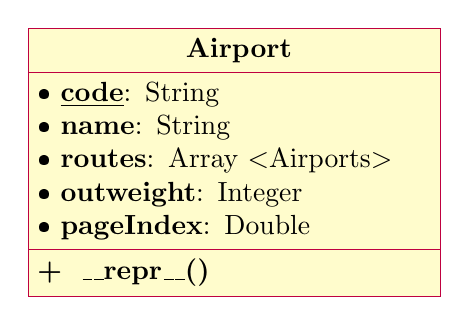
\begin{tikzpicture}
    \begin{class}[text width = 5cm]{ Airport }{0 ,0}
        \attribute {\textbullet \  \textbf{\underline{code}}: String}
        \attribute {\textbullet \ \textbf{name}: String}
        \attribute {\textbullet \ \textbf{routes}: Array \textless Airports\textgreater}
        \attribute {\textbullet \ \textbf{outweight}: Integer}
        \attribute {\textbullet \ \textbf{pageIndex}: Double}
        \operation {\textbf{+ \ \_\_repr\_\_()} }
    \end{class}
    \end{tikzpicture}
    \hspace{5pt}
    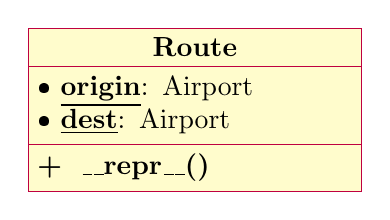
\begin{tikzpicture}
    \begin{class}[text width = 4cm]{Route}{0 ,0}
        \attribute {\textbullet \  \textbf{\underline{origin}}: Airport }
        \attribute {\textbullet \  \textbf{\underline{dest}}: Airport }
        \operation {\textbf{+ \ \_\_repr\_\_()} }
    \end{class}
    \end{tikzpicture}
\caption{Class diagrams}
\label{fig:uml}
\end{figure}

\\\noindent Each attribute of the \textbf{airport} consists of:
\begin{itemize}
    \item \textbf{code}: IATA airport code. Identifier of the airport.
    \item \textbf{name}: Airport name.
    \item \textbf{routes}: List of all airports that have a route that points to the current airport. In other words, list of airports that have as a destination this airport.
    \item \textbf{outweight}: Number of departure flights from this airport.
    \item \textbf{pageIndex}: Page-rank index.
\end{itemize}
\noindent As for the Route structure, its structure is way simpler:
\begin{itemize}
    \item \textbf{Origin}: The airport from where the flight takes off.
    \item \textbf{Dest}: The destination airport, where the flight will land on.
\end{itemize}
The \texttt{repr} function in both structures just defines how the airport and route should be defined.

\section{Difficulties and decisions taken}
Implementing the code and understanding the algorithm was pretty straightforward.
\noindent However, we have faced several problems:
\begin{itemize}
    \item \textbf{Duplication of airports as well as airports without IATA code} - This has been thoroughly explained in the Implementation section.
    \item \textbf{Treatment of dangling nodes} - That is, treatment of airports that are acting as destinations, but not as origin of routes, resulting in $outweight = 0$.
    \item \textbf{Pagerank for dangling nodes} - Somewhat affected by the second point.
    \item \textbf{Proper number of iterations} - Constant number vs. Convergence. 
\end{itemize}

\subsection{Dangling nodes}
Our main difficulty was dealing with the \textit{airports} without departures, that is, the dangling nodes.
There are three accepted approaches for treating nodes with no outgoing edges\cite{pageRank}:
\begin{enumerate}
    \item \textbf{Eliminate} such nodes from the graph (iteratively prune the graph until reaching a steady state). 
    \item Consider such nodes to\textbf{ link back} to the nodes that link to them.
    \item Consider such nodes to \textbf{link to all the other nodes} (effectively making an exit out of them equivalent to a random jump).
\end{enumerate}

The first approach can lead to loss of information. Consider the graph in figure [\ref{graph:s0}] that represents our network. If we prune the graph after 2 iterations we can see that we have lost a lot of information, namely in this case a \textbf{total of 3 airports}. So we have discarded this option.

\usetikzlibrary{arrows, automata, positioning}
\begin{figure}[h!]
    \begin{minipage}{0.24\textwidth}
    \scalebox{0.7}{
    \begin{tikzpicture}[
            > = stealth, % arrow head style
            shorten > = 1pt, % don't touch arrow head to node
            auto,
            node distance = 2cm, % distance between nodes
            semithick % line style
        ]
    
        \tikzstyle{every state}=[
            draw = black,
            thick,
            fill = white,
            minimum size = 4mm
        ]
    
        \node[state] (TLV) {$TLV$};
        \node[state] (BCN) [right of=TLV] {$BCN$};
        \node[state] (KOA) [below  of=BCN] {$KOA$};
        \node[state] (SYD) [below of=TLV] {$SYD$};
        \path[->] (TLV) [] edge node { } (BCN);
        \path[->] (BCN) [] edge node { } (KOA);
        \path[->] (KOA) [] edge node { } (SYD);
    \node[above,font=\bfseries] at (current bounding box.north) {Initial state\\};
    \end{tikzpicture}}
    \end{minipage}
    \begin{minipage}{0.24\textwidth}
    \scalebox{0.7}{
    \begin{tikzpicture}[
            > = stealth, % arrow head style
            shorten > = 1pt, % don't touch arrow head to node
            auto,
            node distance = 2cm, % distance between nodes
            semithick % line style
        ]
    
        \tikzstyle{every state}=[
            draw = black,
            thick,
            fill = white,
            minimum size = 4mm
        ]
    
        \node[state] (TLV) {$TLV$};
        \node[state] (BCN) [right of=TLV] {$BCN$};
        \node[state] (KOA) [below  of=BCN] {$KOA$};
        
        \path[->] (TLV) [] edge node { } (BCN);
        \path[->] (BCN) [] edge node { } (KOA);
        \node[above,font=\bfseries] at (current bounding box.north) {1st iteration - remove SYD};
    \end{tikzpicture}
    }
    \vfill
    \end{minipage}
    \begin{minipage}{0.24\textwidth}
    \scalebox{0.7}{
    \begin{tikzpicture}[
            > = stealth, % arrow head style
            shorten > = 1pt, % don't touch arrow head to node
            auto,
            node distance = 2cm, % distance between nodes
            semithick % line style
        ]
    
        \tikzstyle{every state}=[
            draw = black,
            thick,
            fill = white,
            minimum size = 4mm
        ]
    
        \node[state] (TLV) {$TLV$};
        \node[state] (BCN) [right of=TLV] {$BCN$};
        
        \path[->] (TLV) [] edge node { } (BCN);
                \node[above,font=\bfseries] at (current bounding box.north) {2nd iteration - remove KOA};
    \end{tikzpicture}}
    \end{minipage}
    \begin{minipage}{0.24\textwidth}
    \scalebox{0.7}{
    \begin{tikzpicture}[
            > = stealth, % arrow head style
            shorten > = 1pt, % don't touch arrow head to node
            auto,
            node distance = 2cm, % distance between nodes
            semithick % line style
        ]
    
        \tikzstyle{every state}=[
            draw = black,
            thick,
            fill = white,
            minimum size = 4mm
        ]
        \node[state] (TLV) {$TLV$};
        \node[above,font=\bfseries] at (current bounding box.north) {3rd iteration - remove BCN};
    \end{tikzpicture}
    }
    \end{minipage}
    \caption{1st approach}
    \label{graph:s0}
\end{figure}



\noindent The second and third approaches are more robust and ensure not losing information.
However, applying the second option would be creating false routes that are, in fact, not real, since the graph is directed for a reason: taking into account the direction of routes. In other words, by applying it  we would be biasing the data too much by creating new routes that do not exist, thus the resulting pagerank would be incorrect.

This leaves us with the third option, which is the more reasonable one  with the problem at hand.  W\textbf{e have decided to add edges to all the disconnected nodes to take into account random jumps} (for example, changing the route when doing an scale in an airport). 

As implementation detail it worth mention that we don't keep this new edges on the data structure itself, but we have instead added it to the iterative computation of the pagerank algorithm. Therefore, effectively not having to store  $n^2$ new edges, where $n$ is the number of dangling nodes.

\subsection{Pagerank for dangling nodes}
Although normalizing weights by itself was not difficult for the \textit{normal} nodes (i.e. nodes that were not dangling), we had to consider how to compute the pagerank for the dangling nodes taking them as a special case on each iteration.

\noindent This ended up by treating their pagerank separately with the well-connected ones:
\begin{enumerate}
    \item Let $d$ be the number of dangling nodes. That is, the nodes with outweight 0.
    \item Let $n$ be the total number of nodes.
    \item $prDangNodes = L * \frac{d}{n}$
    \item $evDangNodes = \frac{1}{n}$
    \item for each iteration
    \begin{itemize}
        \item $evDangNodes = prDangNodes * evDangNodes + \frac{1 - L}{n}$
    \end{itemize}
\end{enumerate}


\section{Experiments}
The last step of this project has been performing some experiments.

\subsection{Convergence}
During the implementation of this project, we started with a small number of iterations: only 10.

\noindent After ensuring that the pagerank algorithm was working correctly, we then addressed the suggestion of using a convergence parameter to act as a flag to stop computing the pagerank after reaching a threshold in terms of difference between one pagerank vector $P$ and the new computed one.


The threshold stablished is of value  $1e^{-8}$.  This convergence has led us to a total of 14 iterations. If we check the convergence factor for each iteration, with a static damping factor of 0.85, we can see that we are working with very small units:
\begin{center}
        \includegraphics[width=0.75\linewidth]{plot_conv.png}
        \captionof{figure}{Convergence factor diff. for each iteration}
\end{center}


\subsection{Different dumping factors}

TODO

\subsection{Efficiency}
As a side note, we have noticed that our algorithm is not as fast as we would like it to. With the convergence flag (thus, 14 iterations) it takes a total (on average) of 13 seconds. Almost a second per iteration!

Using the library \texttt{cProfile} we have pinpointed our problem: using the structure provided by the problem, 
we have a bottleneck in times of execution when computing the overall sum of the pagerank for a given airport. 

For context:

\begin{lstlisting}[language=Python,  breaklines=true, numbers=left,   frame=single]
def computeSumDestVert(P, n, i):
    overallSum = 0

    # Iterate through routes that have i as destination
    for e in airportList[i].routes:
        j_code = e.origin
        w_j_i  = e.weight
        airport_j = airportHash.get(j_code)
        j = airportList.index(airport_j)
        overallSum += P[j] * w_j_i / airport_j.outweight
\end{lstlisting}

In line 9 we have the bottleneck. We are getting the index of an airport to specify its position on the vector of pageranks $P$. However, to get this index we need the whole object, which is what we are retrieving on line 8.

This is caused by the structure used. If we were using an adjacency matrix, this problem could be avoided, since we would be working with indexes directly.

Although the bottleneck is minimal with the current data, for future work it would be useful to reimplement this part using a more efficient structure or strategy.

\section{Conclusions}
The conclusions we have arrived to after doing this project are manifold:
\begin{itemize}
    \item The iterative algorithm for pagerank is effective and somewhat efficient for the data at hand. A future work could check the scalability: how efficient would it be with a billion nodes and million nodes? For example.
    \item \textbf{Dangling nodes have to be taken into account} and affect a lot pagerank. We didn't take them into account on our first pagerank computations and thus, the sum of all pageranks did not amount to 1. 
    \item Choosing an right solution for the dangling nodes should be top priority. In our case since the number of nodes was not that large we could opt for the solution of linking all nodes. However, there may be easier cases (computationally speaking) where linking back the nodes to the ones they are coming makes sense.
    \item Using a convergence of $1e^{-8}$ leads in our case to a total number of 14 iterations, which is not that far from what we started on: 10 iterations.
\end{itemize}

\nocite{*}
\bibliographystyle{unsrt}
\bibliography{references}
\end{document}
